% Nallino, Part II p. 252: the obliquity of the epicycle of Venus or Mercury, redrawn from the print at the size of
% the print. The coordinates are those of a 400 dpi render of the figure (crop from x 118 pt, y 378 pt of the master
% page; y downward). The epicycle has its centre in H and its true apogee in Q, on the line QHE to the Earth E; T is
% the planet, N the foot of its perpendicular on QH, M the foot of its perpendicular on the plane of the deferent.
% NM and TM are dashed, ME dotted, as on the print.
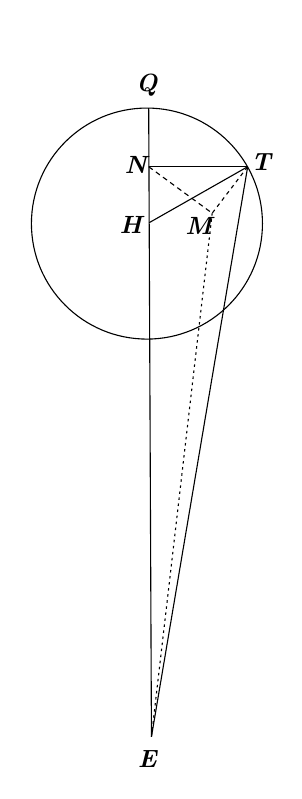
\begin{tikzpicture}[x=0.0635mm,y=-0.0635mm,line width=0.4pt,every node/.style={font=\bfseries\itshape\small,inner sep=1pt}]
\path (40,-30);
\coordinate (H) at (283,360);
\coordinate (N) at (282,248);
\coordinate (T) at (480,248);
\coordinate (M) at (409,341);
\coordinate (E) at (287.5,1388);
\draw (278.5,361.75) circle[radius=231];
\draw (282,130.75) -- (E);
\draw (N) -- (T);
\draw (H) -- (T);
\draw (T) -- (E);
\draw[dash pattern=on 1.8pt off 1.4pt] (N) -- (M);
\draw[dash pattern=on 1.4pt off 1.4pt] (T) -- (M);
\draw[dash pattern=on 0.9pt off 1.3pt] (M) -- (E);
\node at (278,86) {Q};
\node at (256,244) {N};
\node at (506.5,239) {T};
\node at (246,365) {H};
\node at (382,366.5) {M};
\node at (279,1433) {E};
\end{tikzpicture}
